\section{Outdoor localization}
\label{subseq:outdoor}

\begin{table}
	\centering
	\begin{scriptsize}
	\begin{tabular}{c l | c c c c c c }
					&	&	Great Court	&	Kings C.	&	Old Hosp.	&	Shop &	St Mary's &	Street \\
		\hline	
	\multirow{2}{*}{{Im. retrieval}}
	& FC-unsup.  	& 27.6/26.79 & 4.4/6.10 & 6.2/10.09 & 4.3/14.93	& 6.9/15.17 & 95.5/58.38 \\
	& C+LSTM-unsup 	& 24.3/20.94 & 5.0/5.86 & 6.5/8.60	& 3.2/9.47  & 5.9/12.71	& 92.5/67.10 \\
	\multirow{2}{*}{{PnlP}}
	& FC-unsup. 	& 25.5/22.64 & 2.9/2.98 & 4.9/6.37 & 1.8/5.78 & 3.5/6.99 & 76.2/51.91 \\
	& C+LSTM-unsup 	& 13.2/10.07 & 2.7/3.10	& 3.5/5.55 & 1.1/3.38 & 2.6/5.85 & 69.5/52.07 \\[1pt]
	\hline
	& {Posenet~\citep{Kendall2017}} & - & 0.9/1.04 & 3.2/3.29 & 0.9/3.78 & 1.6/3.32 & 20.3/25.5 \\
	\end{tabular}
	\end{scriptsize}
	\caption[Pose refinement results on outdoor dataset]{\label{tab:outdoor} Results on the Cambridge Landmarks~\citep{Kendall2015} outdoor dataset, we report median position/orientation error in meters/degree. We compare our two network architectures, FC and C+LSTM, trained in an unsupervised manner.}
\end{table}


As mentioned previously, we only test our unsupervised set-up for outdoor image pose estimation as the Cambridge Landmarks dataset~\citep{Kendall2015} does not contain ground truth depth maps. Results are presented in table~\ref{tab:outdoor}. PnlP performs well on outdoor scene, with a mean improvement of $\times$1.3/$\times$1.4 for FC architecture, and $\times$1.5/$\times$1.6 for C+\ac{lstm}, in position/rotation precision over initial pose given by \ac{cbir}. Superior performances of C+\ac{lstm} model can be explained by a better capability of the recurrent cells in the C+\ac{lstm} decoder for modeling the 3D structure of the scene, as shown in figure~\ref{fig:depth_map_outdoor}. Our method is not able to recover a proper pose for the scene Street. As same as for the indoor failure case, this is the result of a poor initial pose estimation at the CBIR preliminary step. Compared to Posenet~\citep{Kendall2017}, our method is marginally less precise but requires only one trained model compared to the 6 models needed by Posenet and can potentially be used on unknown scenes according to the previous indoor experiments. We do not compare our method to Relocnet~\citep{Purkait2018} baseline because authors do not evaluate Relocnet on outdoor scenes.


\begin{landscape}
\begin{figure}
    \centering

	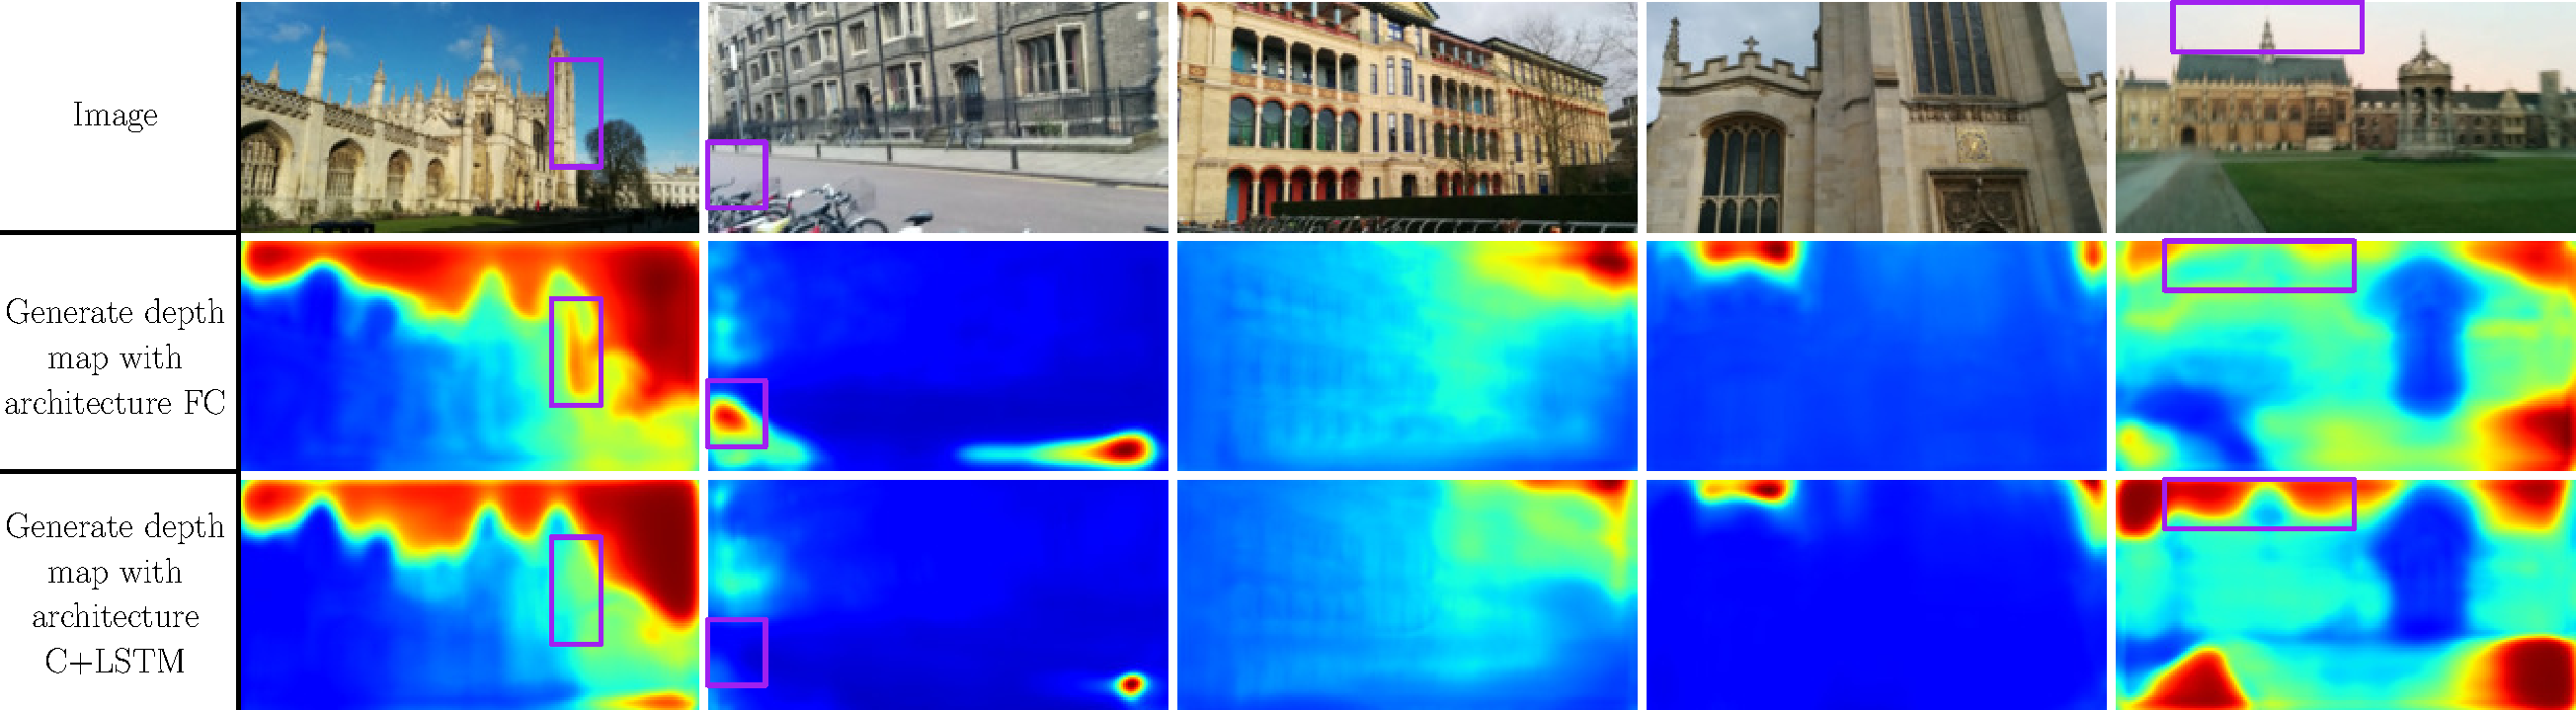
\includegraphics[width=\linewidth]{results/outdoor/depth_maps}
	\caption[Generated outdoor depth maps]{\label{fig:depth_map_outdoor} Visualisation of the depth map generated from RGB input by our two architectures, FC and C+LSTM, trained in an unsupervised manner on Cambridge Landmarks dataset~\citep{Kendall2015}. \textcolor{purple}{Purple boxes} show regions where C+LSTM network produces slightly better depth map reconstruction compared to FC.}
	
\end{figure}
\end{landscape}